% Discussion / AST
% Andreas
\section{AST}
TODO:
 * Rewrite rules + operators: lett a forandre, flytte rundt paa ting
 * Bygge subtraer med imaginaere noder eller tokens
 * Problematisk aa generere parser uten AST-kode naar regler+operatorer forst har
   blitt addet
 * Problematisk med JFlex/CUP, mye arbeid
 * Tredjeparts verktoy med JavaCC
 * Expressing FLWOR, full-text, path expressions
 * Mulighet for dataflytanalyse, typesjekking, symboltabell
 
The rewrite rules and operators (described in section
\ref{sect:results:parser_output_ast}) made it easy to change and restructure the
AST output from ANTLR. In a intuitive way, they were used to construct subtrees
using both real and imaginary tokens, as described in section
\ref{sect:impl:ast}. Contrast this to JFlex/CUP, one of the alternative
parser generators evaluated in this project (see section
\ref{sect:method:alternatives}), where the AST construction has to be done
manually from scratch by adding action code to the grammar instead of simple
rewrite rules. However, this ease of change may makes it easy to break implicit
API contracts with other programs. A good starting point could be to study other
XQuery implementations and their respective AST structures. 

One notable problem with the rewrite rules in ANTLR is the fact that after they
have been added to the grammar, it is no longer possible to generate a parser
which does not produce an AST (by omitting the \verb!output=AST! option). ANTLR will
instead refuse to generate a parser and output syntax error messages since the rewrite
rules are no longer recognized.

The current AST output from ANTLR seems to be well suited for traversion and data
flow analysis, which is a requirement for implementation of type checking,
proper scoping and symbol tables, as well as optimizations and transformations
to new structures. ANTLR is capable of producing ``tree parsers'' (see
\cite{definitiveAntlr}, section 3.3) based on rewrite rules, so it may be
possible to utilize ANTLR even further to achieve a tree
parser without writing one from scratch.

In section \ref{sect:results:parser_output_ast}, we demonstrated the AST output
capabilities of our resulting parser. In figure \ref{tree:ast:flwor1}, an
example with a FLWOR query was presented. In this example there is a path
expression (\verb!/bookstore/book/title!, which is also used in the example in
figure \ref{tree:ast:pathexpr}) encoded as seen in figure
\ref{fig:discussion:ast:path1}. 

\begin{figure}[h!]
\centering
 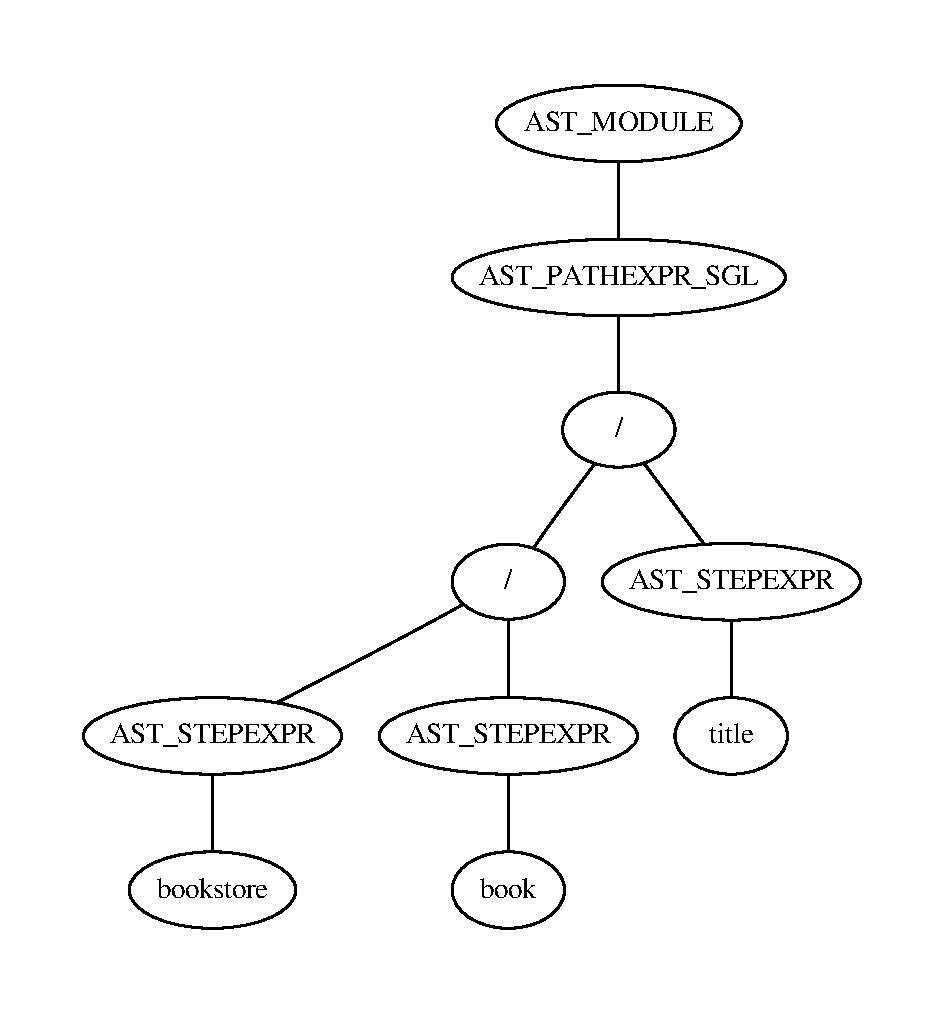
\includegraphics[width=0.4\textwidth]{img/graphs/path1}
\caption{Generated AST tree for a simple path expression}
\label{fig:discussion:ast:path1}
\end{figure}


Generelle resultat, bra/d\aa rlig (AST) \#\# typesjekking (bedre \aa~gj\o re
p\aa~AST'en) -> putt i egen section i discussion -------v 
symtabs (bedre \aa~gj\o re p\aa~ AST'en))

Gjorde vi riktige valg? Ble ting som forventet? Hva hadde skjedd om vi brukte alternativ m\aa te? 

\underline{\textbf{\LARGE //ODOT:}}